\section{Алгоритм поиска путей с КС ограничениями}
\label{section:algo_impl}

В данной секции предлагается рассмотреть основные детали реализации алгоритма~\cite{inbook:kronecker_cfpq_adbis} поиска путей с КС ограничениями через тензорное произведение на GPU с использованием библиотеки cuBool, особенности реализации которой были представлены в предыдущей главе..

Реализация алгоритма написана на языке Python с использованием пакета \textbf{pycubool}.
Программа, исполняемая Python-интерпретатором, задает только последовательность вызовов операций.
Вычислительно-интенсивные части алгоритма выполняются на GPU в рамках библиотеки, 
поэтому решение в целом остается производительным.
 
На вход алгоритм получает граф и КС грамматику. 
Граф представлен в виде булевой матричной декомпозиции матрицы смежности графа.
КС грамматика закодирована в виде рекурсивного автомата. 
Его матрица переходов также представлена в булевой матричной декомпозиции.
На выходе алгоритм возвращает матрицу смежности графа достижимости, а также индекс, 
который позволяет восстанавливать все пути в графе в соответствии с входной грамматикой.

Также с использованием \textbf{pycubool} реализован классический матричный алгоритм Рустама Азимова~\cite{inproceedings:matrix_cfpq}, требуемый для корректного сравнения производительности с алгоритмом на основе тензорного произведения.

Реализации упомянутых алгоритмов доступны в рамках открытого проекта \textbf{CFPQ-PyAlgo}~\cite{net:cfpq_py_algo}.
Данный проект предоставляет инфраструктуру для осуществления замеров производительности, а также для загрузки и конвертации данных, требуемых для экспериментов.
Архитектура данного стенда представлена на рис.~\ref{fig:cfpq_py_algo}. 
Тестовый стенд позволяет использовать различные библиотеки и инструменты для реализации в модуле  \textbf{Algorithms} алгоритмов поиска путей с КС ограничениями. Также стенд предоставляет утилиты для загрузки входных графов в модуле \textbf{Grpah}, для загрузки грамматик и преобразования их в требуемый формат в модуле \textbf{Grammar} соответственно.
Пакет \textbf{CFPQ-Data}~\cite{net:cfpq_data} используется для загрузки из локального или удаленного хранилища актуальной версии набора данных для замеров.

\begin{figure}[]
    \centering
    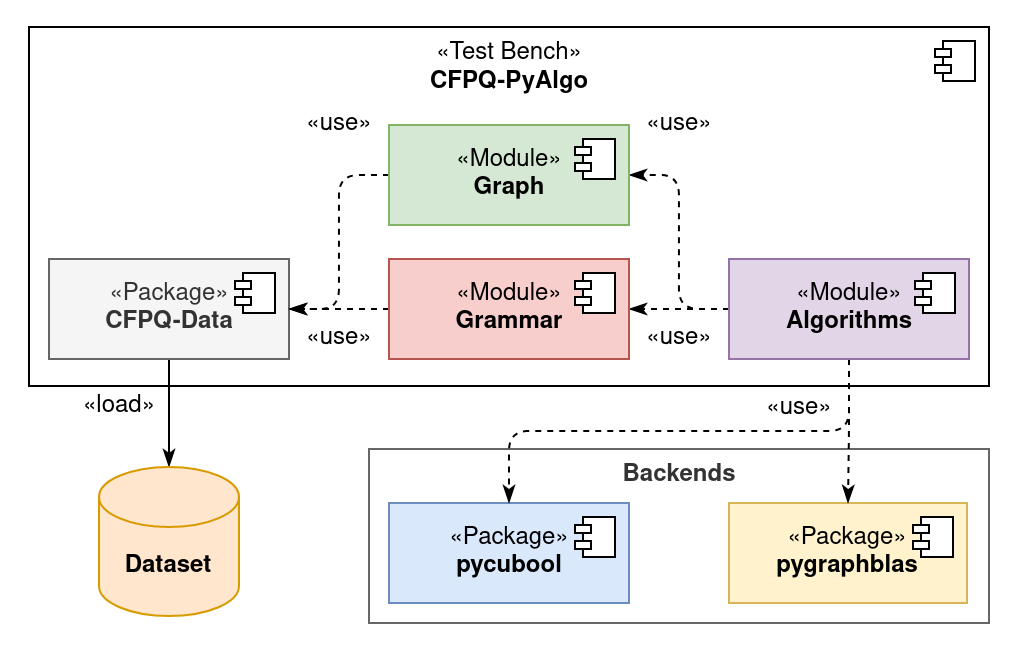
\includegraphics[width=0.9\textwidth]{images/cfpq_pyalgo.png}
    \caption{Архитектура стенда для тестирования алгоритмов}
    \label{fig:cfpq_py_algo}
\end{figure}

В инфраструктуре уже доступны базовые реализации алгоритма Рустама Азимова~\cite{inproceedings:matrix_cfpq} и алгоритма на основе тензорного произведения для вычислений на CPU. 
В качестве основы эти реализации используют пакет \textbf{pygraphblas}, который предоставляет доступ к примитивам разреженной линейной алгебры из стандарта GraphBLAS API~\cite{paper:graphblas_foundations} и его эталонной реализации SuiteSparse~\cite{article:suite_sparse_for_graph_problems}. 
Данные реализации алгоритмов также используются для проведения экспериментального исследования.





